%% Results and discussion
%%=========================================

\chapter{Results and Discussion}
\label{ch:results}
Below are the results for each test ran in our experiments. The results are discussed briefly and summarized in the next chapter.

%%=========================================

\section{Accuracy on Datasets}
Table \ref{table:accuracy_model_data_sets} contains the accuracy for each model on each of the three datasets of various sizes, as described in section \ref{sec:accuracy_on_datasets}. The accuracy and loss plots for each test are presented below, showing the progression over the epochs.

\begin{table}[H]
    \centering
    \begin{tabular}{|l|l|l|l|}
        \hline 
                                        & \textbf{Small dataset}          & \textbf{Medium dataset}         & \textbf{Big dataset}            \\ \hline
        {\tt VecRep }                   & 16.80\%                         & 25.14\%                         & 55.01\%                         \\ \hline
        {\tt EncDecReg}                 & 41.20\%                         & 55.52\%                         & 95.49\%                         \\ \hline
        {\tt EncDecAtt}                 & \textbf{92.00\%}                & \textbf{97.16\%}                & \textbf{98.75\%}                \\ \hline
    \end{tabular}
    \caption{Test accuracy for each model on each test set, with the best results for each test set highlighted}
    \label{table:accuracy_model_data_sets}
\end{table}

The {\tt EncDecAtt} model had the best results on all three datasets, with the lowest accuracy of \(92\%\). For all three datasets, the model had an accuracy of more than \(90\%\), and the difference between the best and worst results were less than \(7\%\). This is in contrast to the {\tt EncDecReg} model, which had low accuracy results for both the small and medium datasets, but high accuracy on the big dataset. The {\tt EncDecReg} model had an accuracy of almost \(95.5\%\), which is less than \(4\%\) worse than the results for the {\tt EncDecAtt} model. The difference in the accuracy between the {\tt EncDecReg} and {\tt EncDecAtt} model on the medium dataset was more than \(40\%\), and almost \(50\%\) on the small dataset. The {\tt VecRep} model had consistently lower accuracy than the two other, but almost doubled its accuracy from the medium to the big dataset.

\subsection{VecRep}
\subsubsection{Accuracy and Loss}
\resultplots{fig/results/experiment1/small/vecrep/}{plot_accuracy_crop.png}{plot_loss_crop.png}{result1_small_vecrep}{Accuracy and loss for {\tt VecRep} on small dataset}
\resultplots{fig/results/experiment1/medium/vecrep/}{plot_accuracy_crop.png}{plot_loss_crop.png}{result1_medium_vecrep}{Accuracy and loss for {\tt VecRep} on medium dataset}
\resultplots{fig/results/experiment1/big/vecrep/}{plot_accuracy_crop.png}{plot_loss_crop.png}{result1_big_vecrep}{Accuracy and loss for {\tt VecRep} on big dataset}

\newpage
\subsubsection{Confusion Matrix}
\begin{figure}[H]
    \centering
    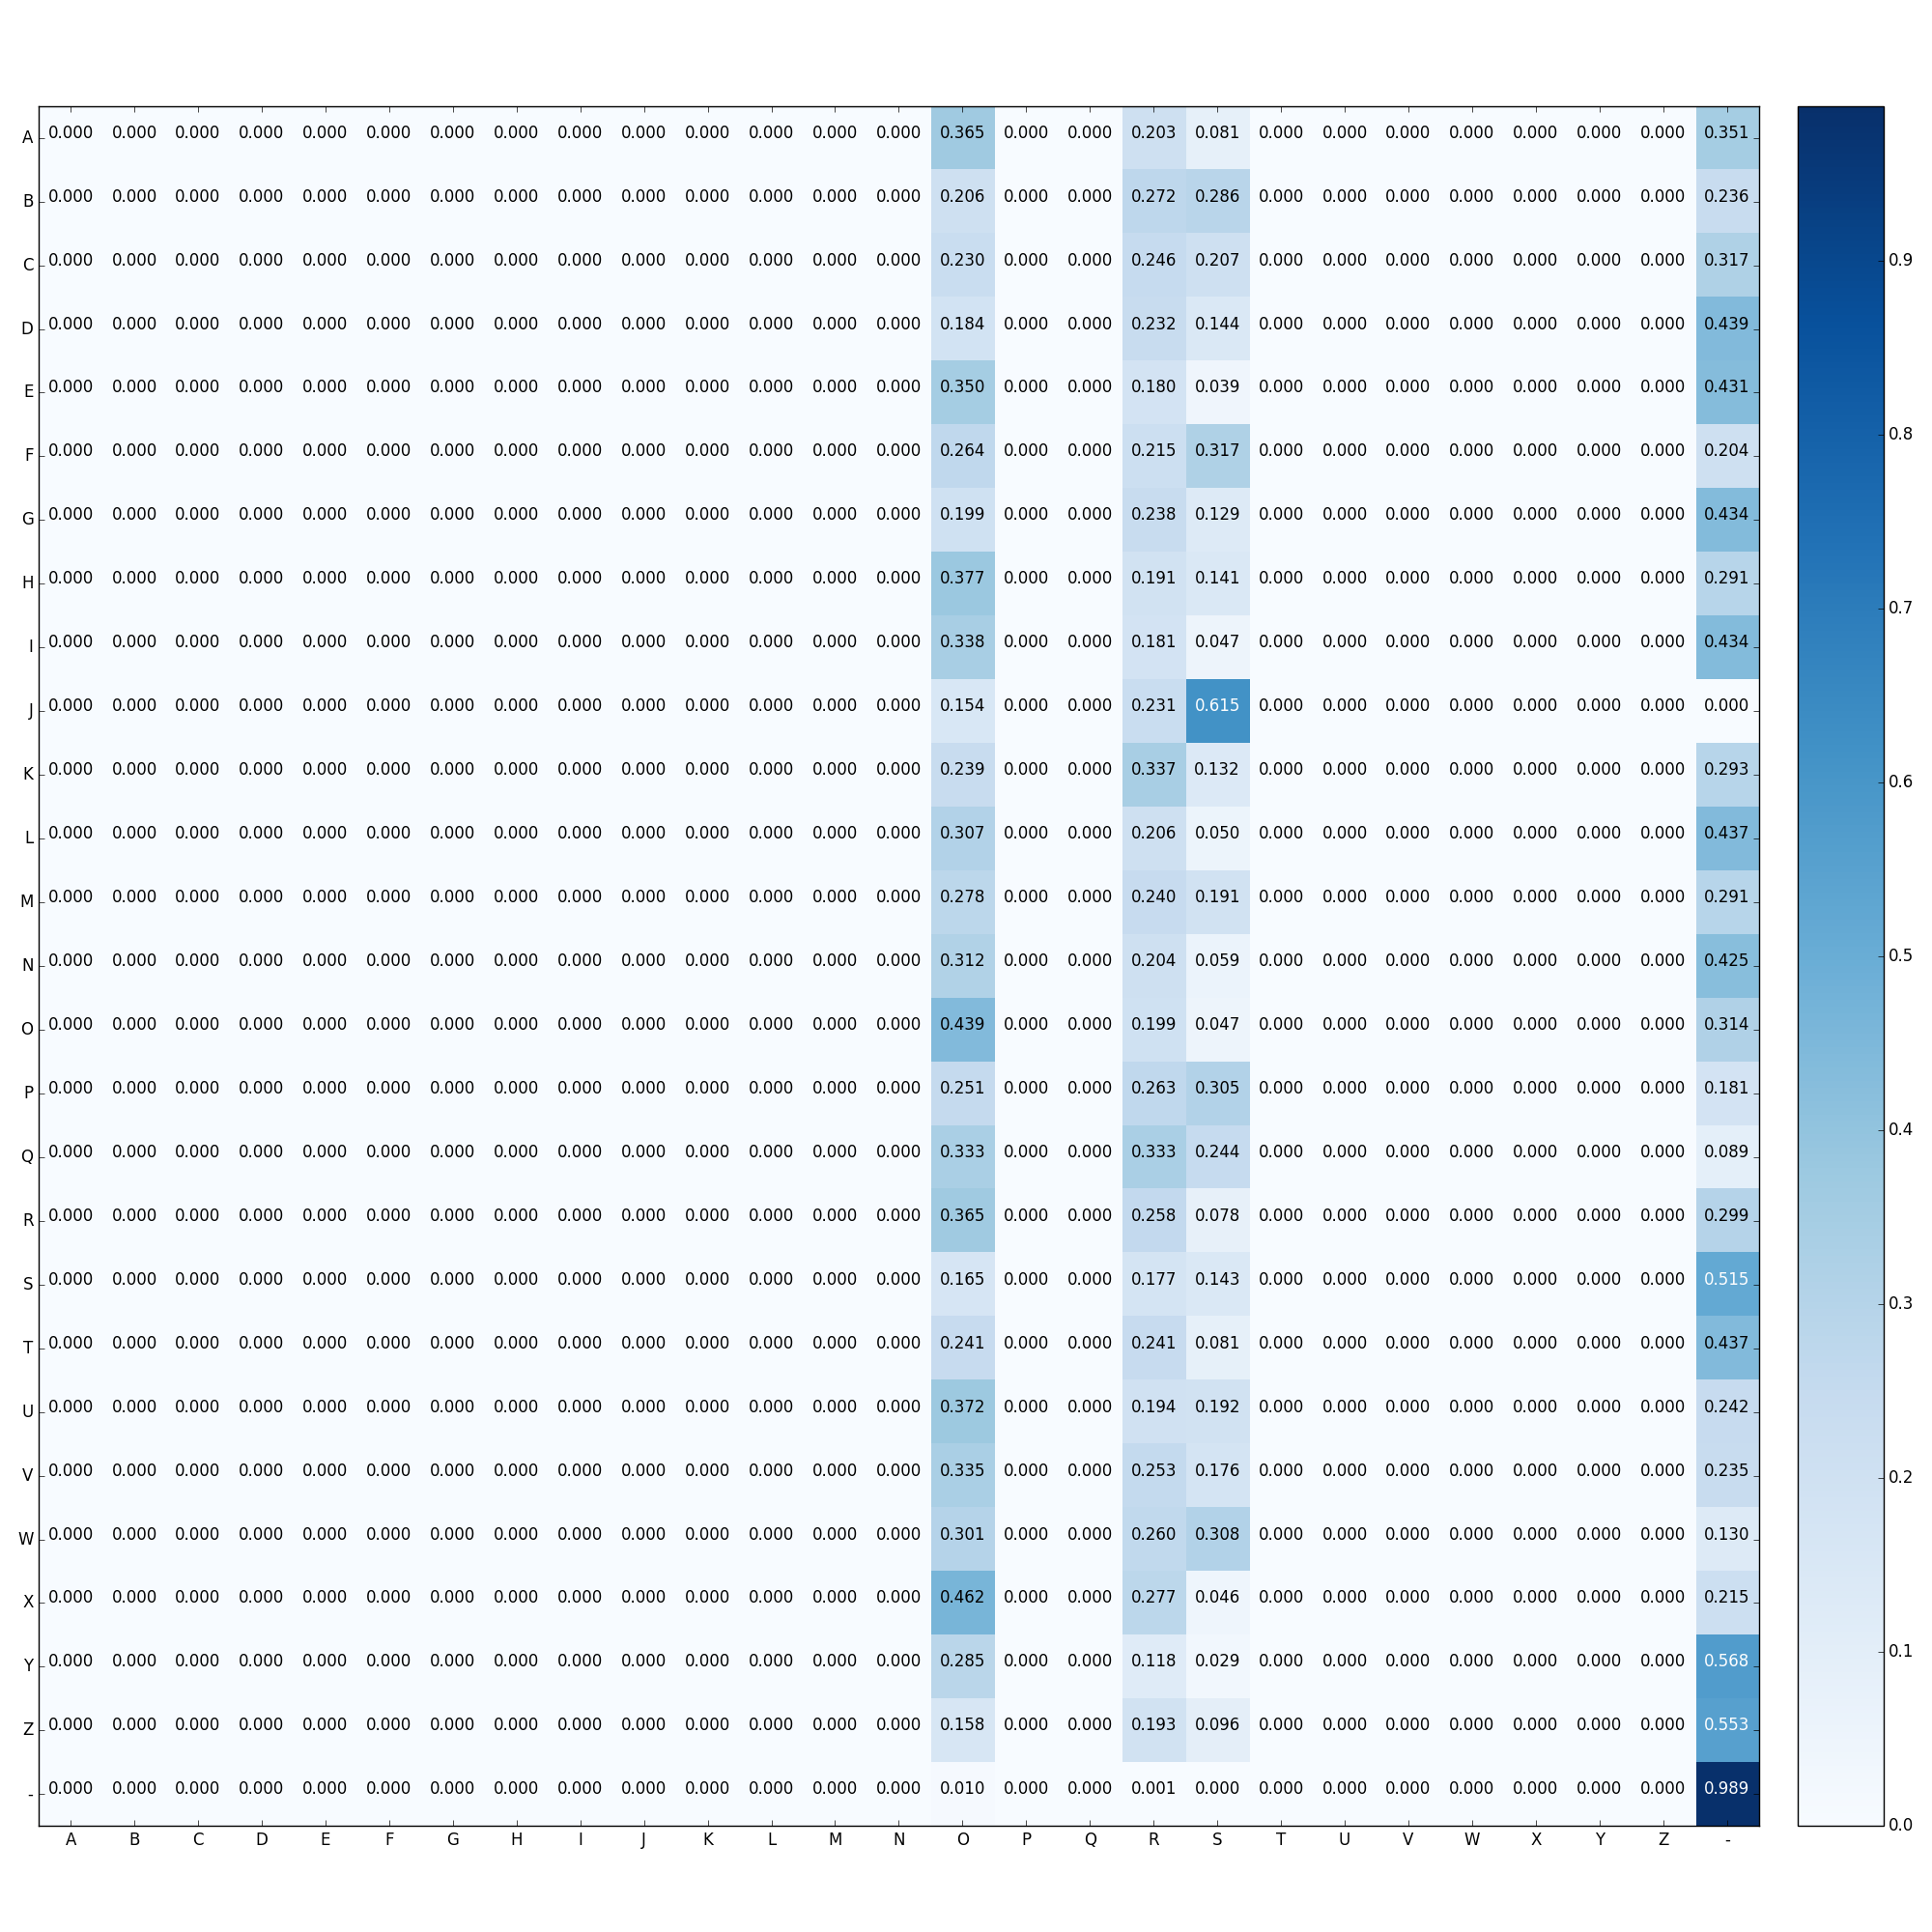
\includegraphics[width=1\textwidth]{fig/results/experiment1/big/vecrep/confusion_matrix.png}
    \caption{Confusion matrix for the best {\tt VecRep} model on the big dataset}
    \label{fig:result1_big_vecrep_confusion_matrix}
\end{figure}

The confusion matrix illustrated in Figure \ref{fig:result1_big_vecrep_confusion_matrix} explains how the model was able to produce an accuracy of over \(50\%\) on the big dataset. The big dataset had a maximum word length of \(20\) letters, while most words in the English language, as well as our datasets, being shorter than this. To compensate for this, the labels were zero-padded to fill the empty output labels. The {\tt VecRep} seem to base its predictions on the most common labels, which would be the padding symbol. It also looks to prefer other common labels such as ``O", ``R", and ``S". Every other cell in the confusion matrix is zero, meaning the model did not predict on more than four of the total 27 classes.

\subsection{EncDecReg}
\subsubsection{Accuracy and Loss}
\resultplots{fig/results/experiment1/small/encdecreg/}{plot_accuracy_crop.png}{plot_loss_crop.png}{result1_small_encdecreg}{Accuracy and loss for {\tt EncDecReg} on small dataset}
\resultplots{fig/results/experiment1/medium/encdecreg/}{plot_accuracy_crop.png}{plot_loss_crop.png}{result1_medium_encdecreg}{Accuracy and loss for {\tt EncDecReg} on medium dataset}
\resultplots{fig/results/experiment1/big/encdecreg/}{plot_accuracy_crop.png}{plot_loss_crop.png}{result1_big_encdecreg}{Accuracy and loss for {\tt EncDecReg} on big dataset}

\newpage
\subsubsection{Confusion Matrix}
\begin{figure}[H]
    \centering
    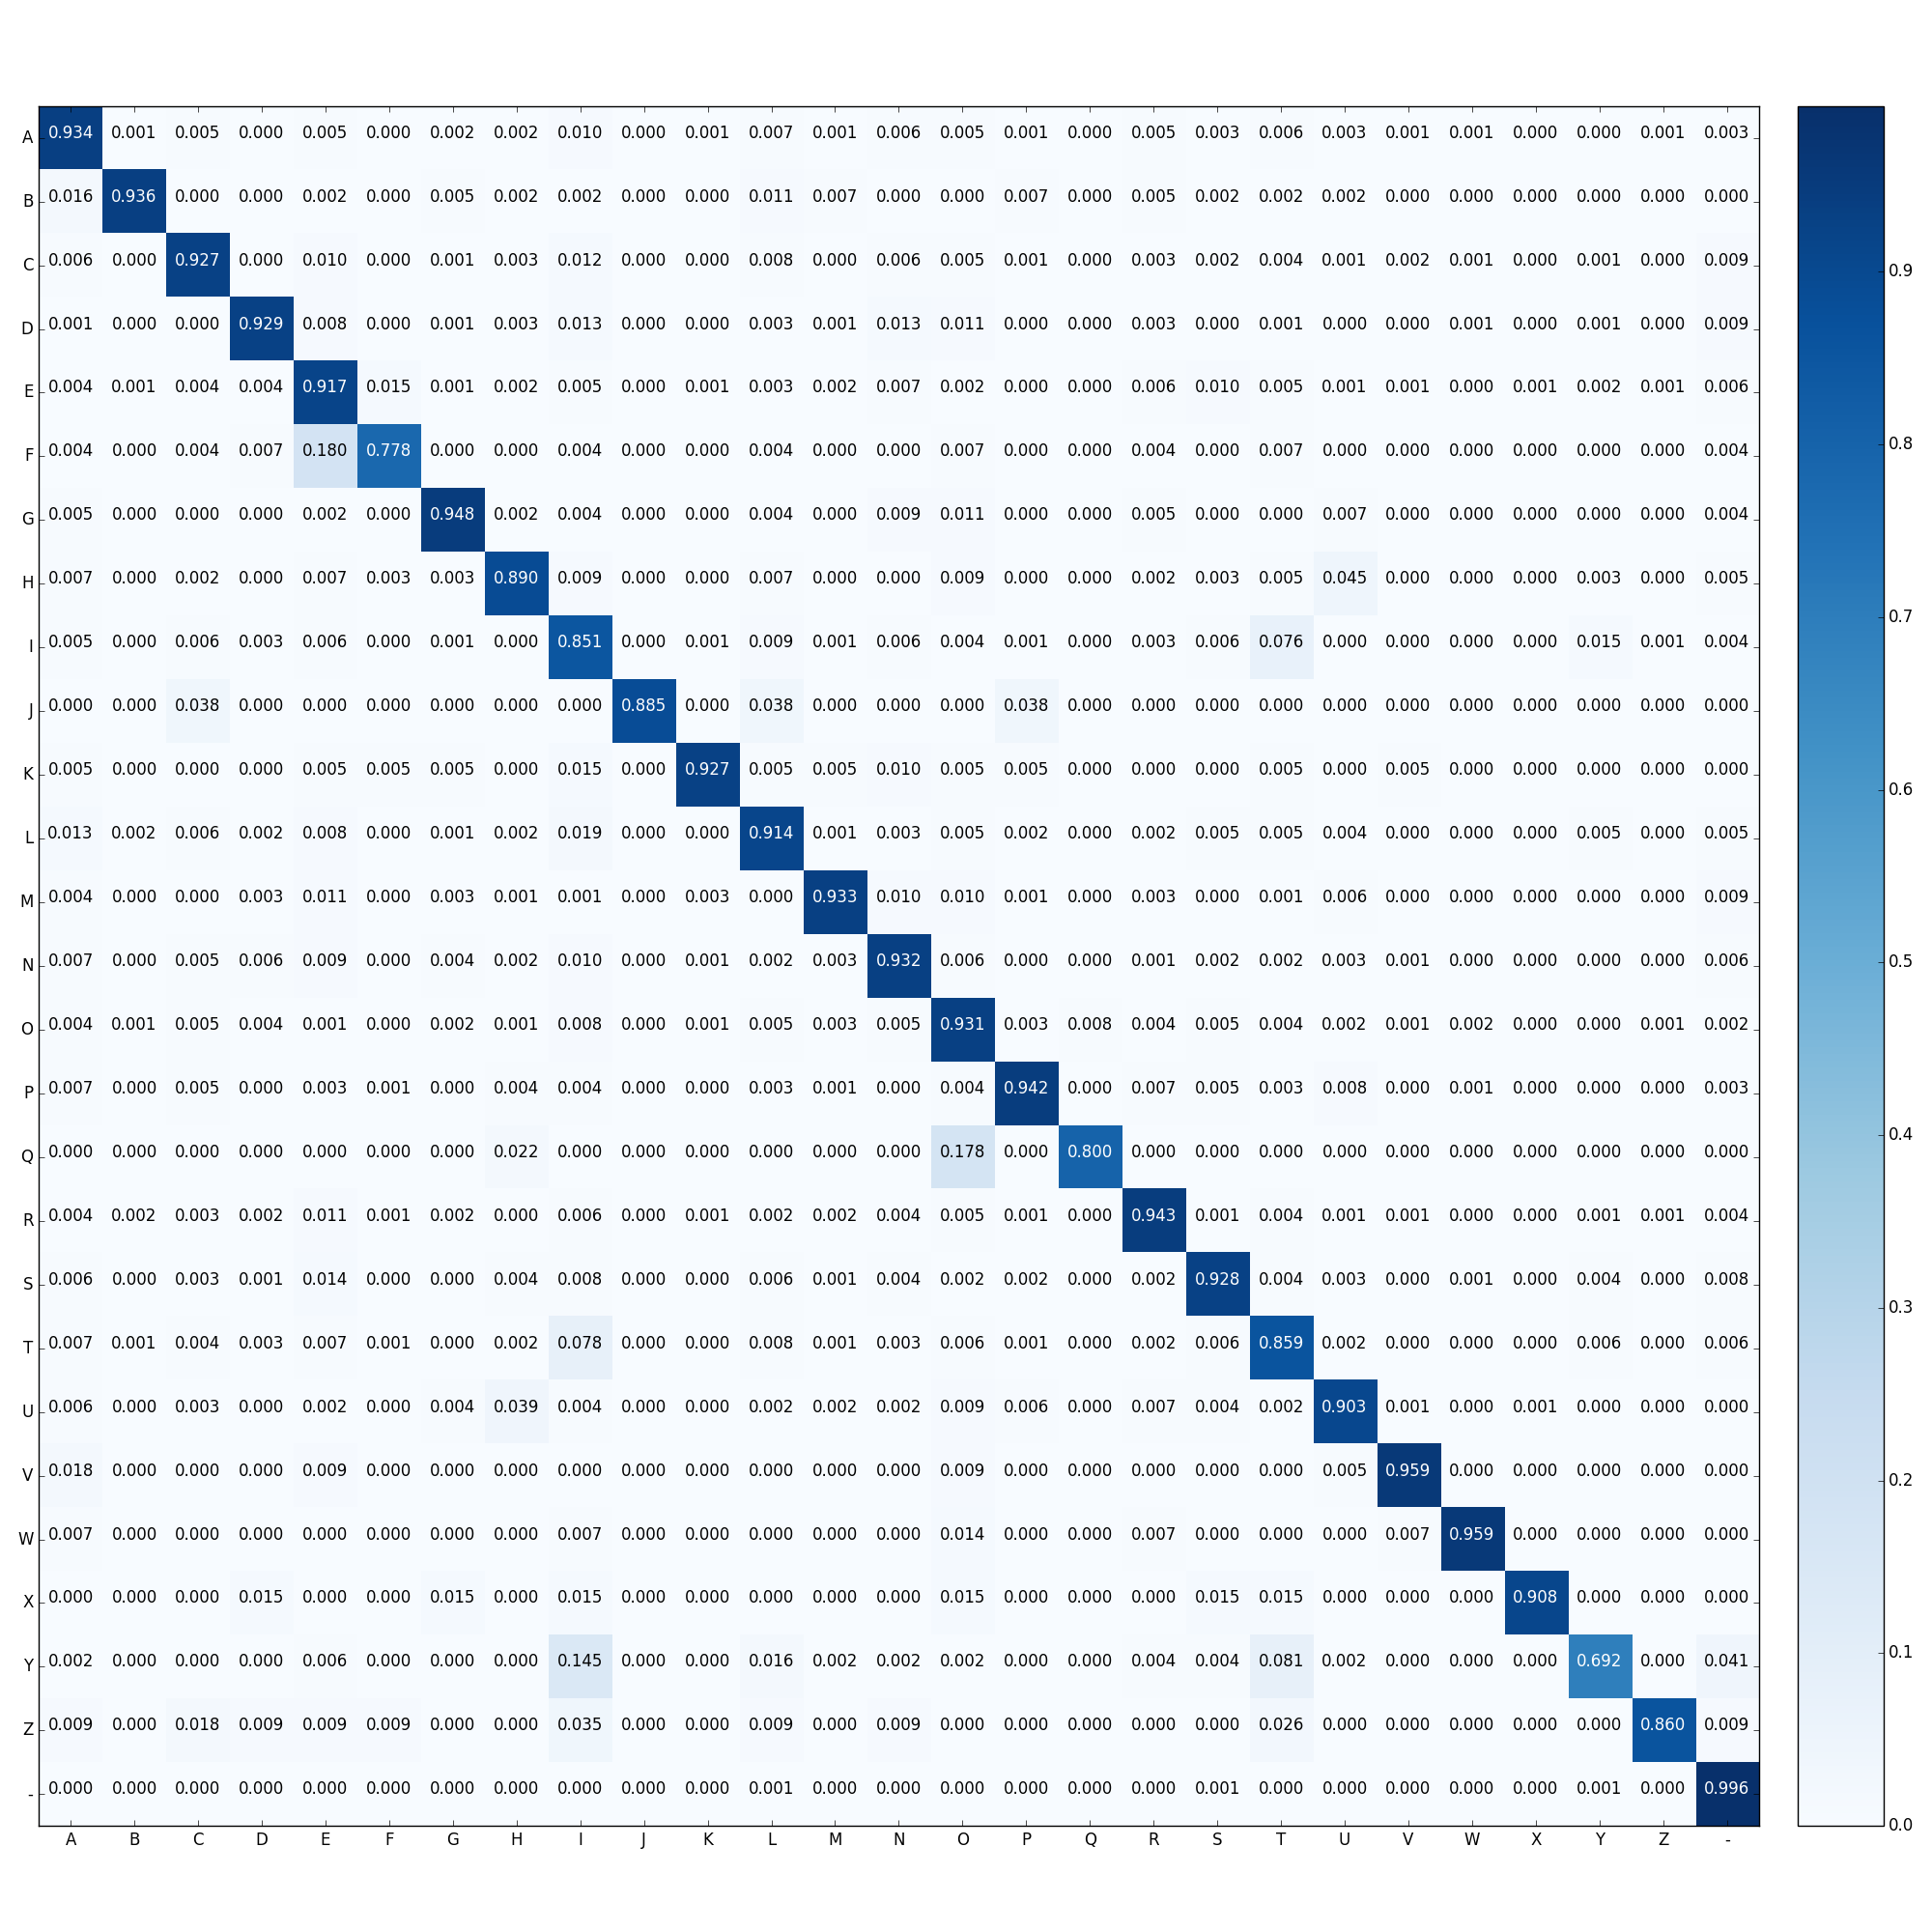
\includegraphics[width=1\textwidth]{fig/results/experiment1/big/encdecreg/confusion_matrix.png}
    \caption{Confusion matrix for the best {\tt EncDecReg} model on the big dataset}
    \label{fig:result1_big_encdecreg_confusion_matrix}
\end{figure}

The {\tt EncDecReg} had an accuracy of almost \(95.5\%\) on the big dataset, which is reflected in the confusion matrix in Figure \ref{fig:result1_big_encdecreg_confusion_matrix}. The confusion matrix has a clearly defined diagonal line with a very high individual accuracy. Most of the labels have an accuracy of over \(0.9\) with a few exceptions. ``Y" is wrongly labeled as an ``I" in \(14.5\%\) of the instances, and as a ``T" in \(8.5\%\) of the instances. The most wrongly labeled classes are ``F" as an ``E" (\(18\%\)) and ``Q" as ``O"  (\(17.8\%\)).

\subsection{EncDecAtt}
\subsubsection{Accuracy and Loss}
\resultplots{fig/results/experiment1/small/encdecatt/}{plot_accuracy_crop.png}{plot_loss_crop.png}{result1_small_encdecatt}{Accuracy and loss for {\tt EncDecAtt} on small dataset}
\resultplots{fig/results/experiment1/medium/encdecatt/}{plot_accuracy_crop.png}{plot_loss_crop.png}{result1_medium_encdecatt}{Accuracy and loss for {\tt EncDecAtt} on medium dataset}
\resultplots{fig/results/experiment1/big/encdecatt/}{plot_accuracy_crop.png}{plot_loss_crop.png}{result1_big_encdecatt}{Accuracy and loss for {\tt EncDecAtt} on big dataset}

\newpage
\subsubsection{Confusion Matrix}
\begin{figure}[H]
    \centering
    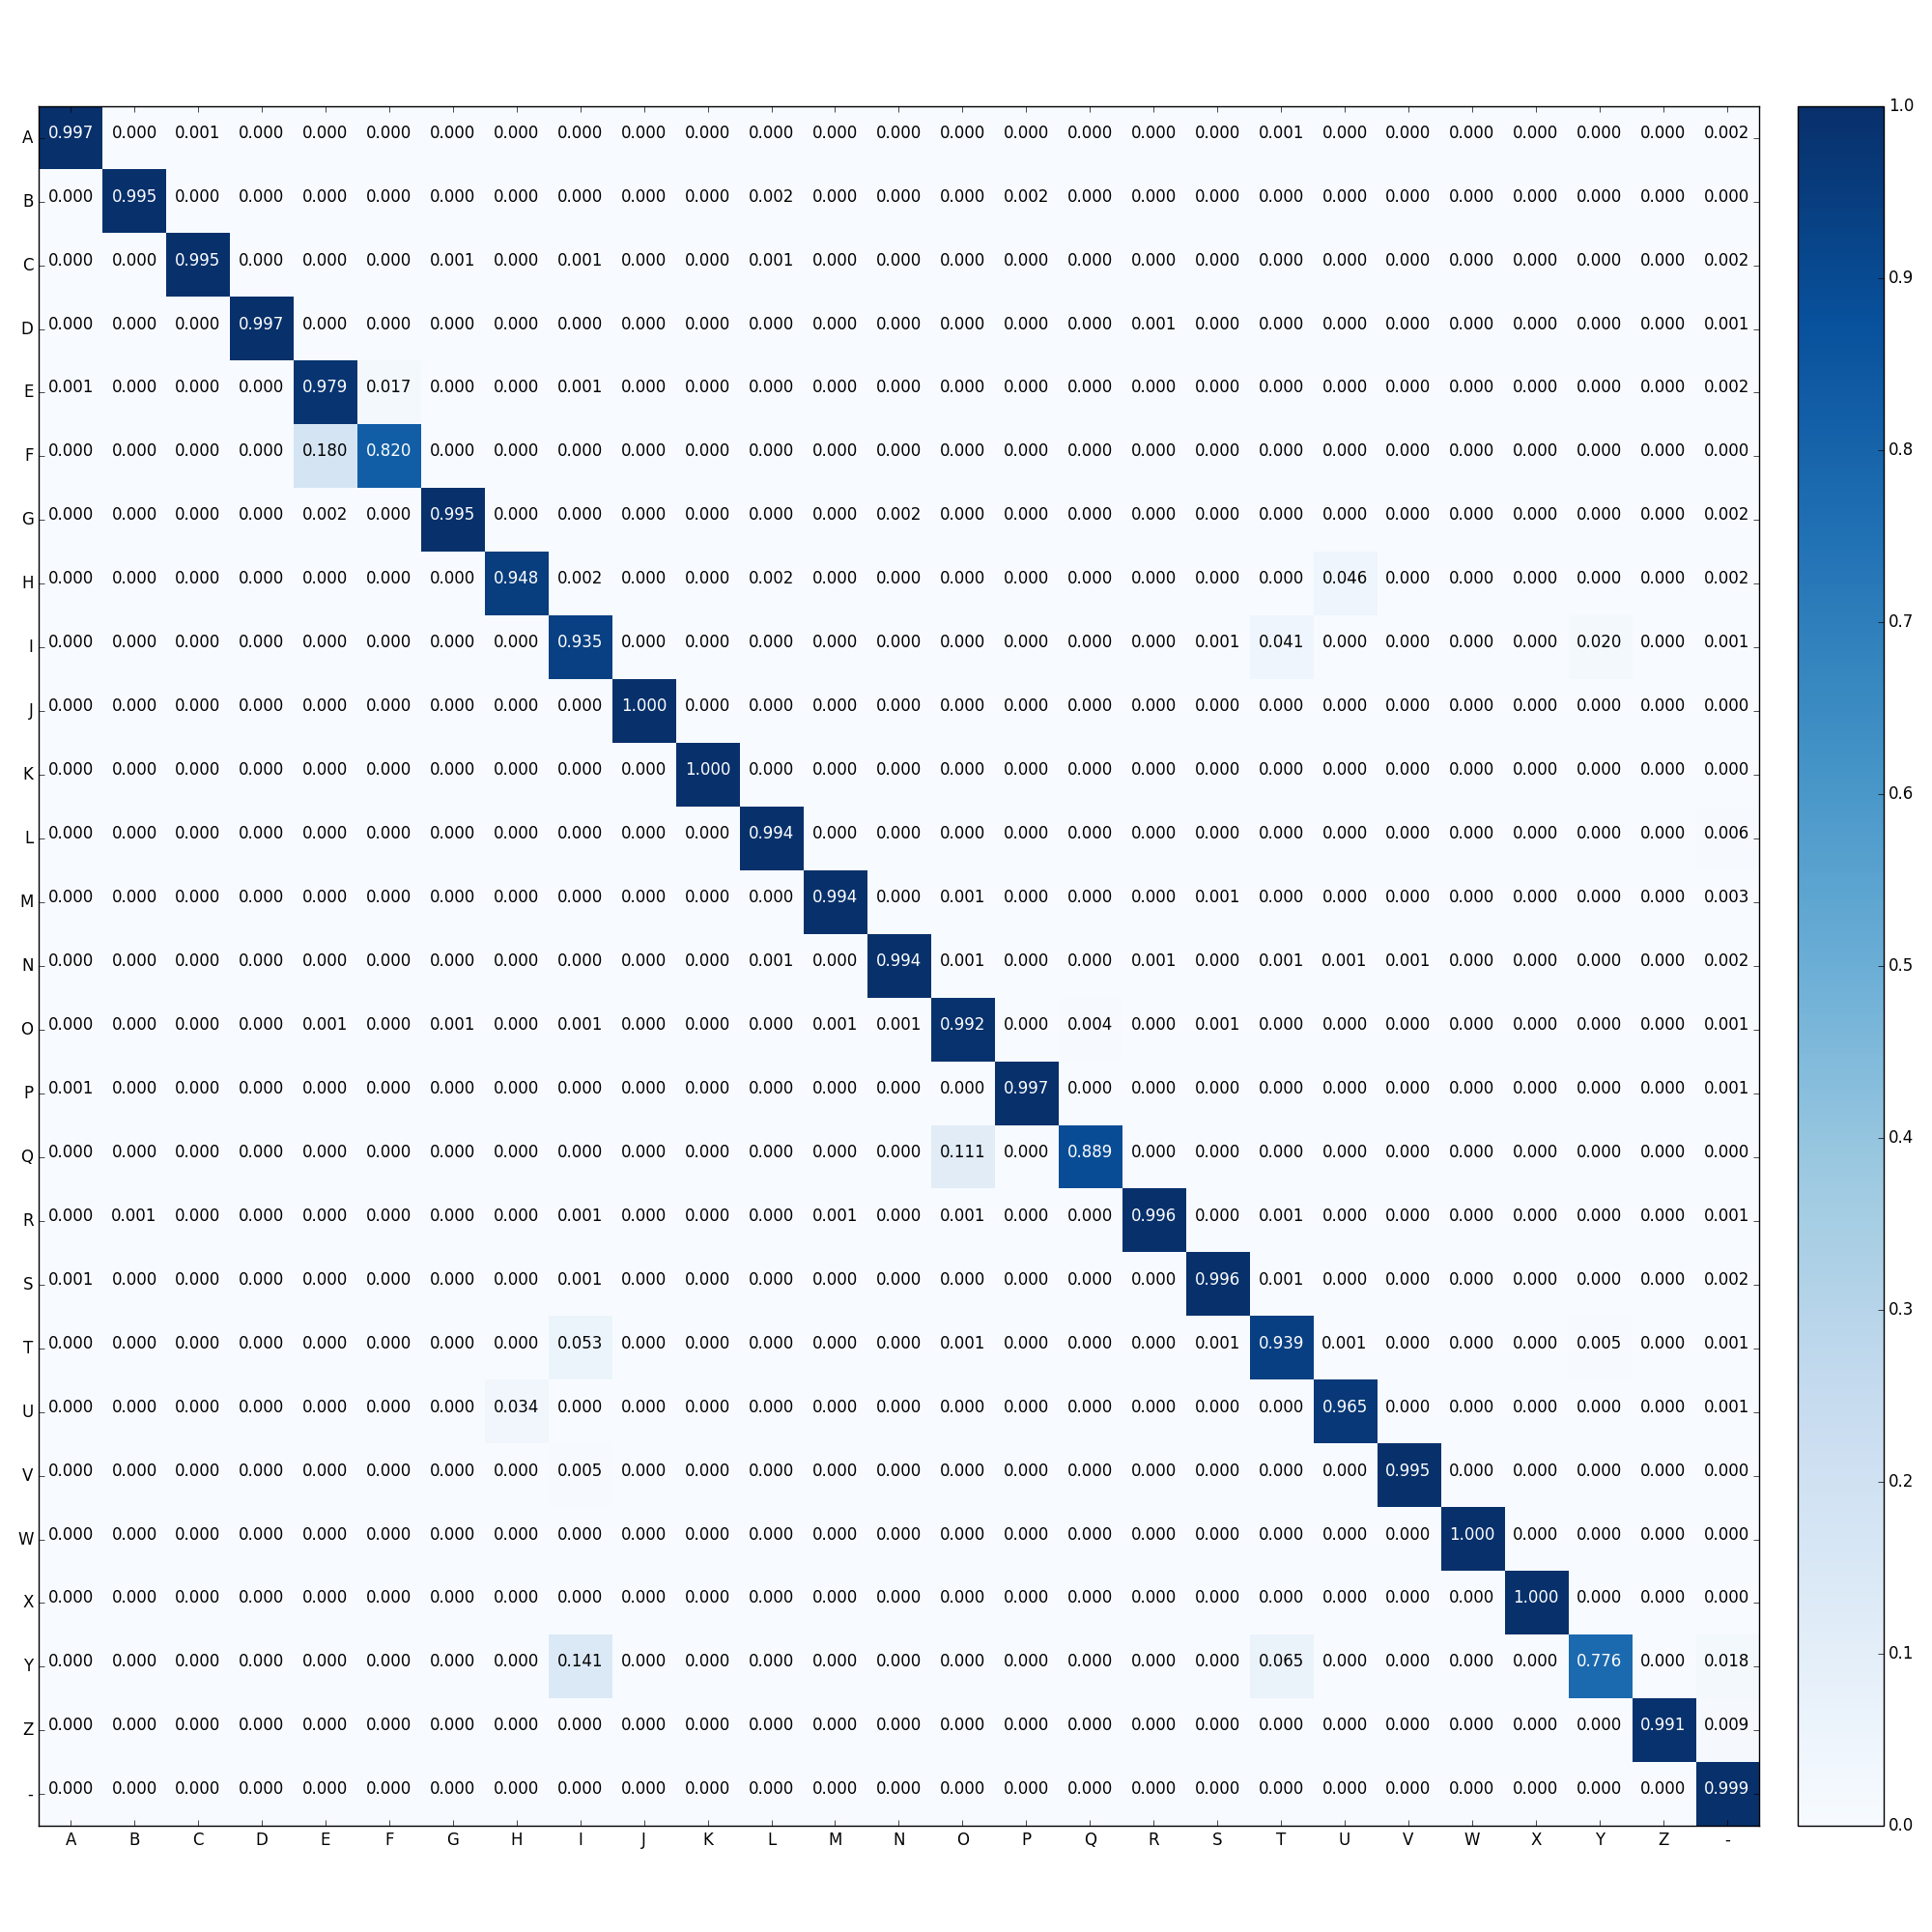
\includegraphics[width=1\textwidth]{fig/results/experiment1/big/encdecatt/confusion_matrix.png}
    \caption{Confusion matrix for the best {\tt EncDecAtt} model on the big dataset}
    \label{fig:result1_big_encdecatt_confusion_matrix}
\end{figure}

The confusion matrix for the {\tt EncDecAtt} model (Figure \ref{fig:result1_big_encdecatt_confusion_matrix}) has high individual accuracy, similar to the results of the {\tt EncDegReg} model, although this model has improved even further. The {\tt EncDegReg} model successfully classifies four classes without a single error, and only three classes have a lower accuracy than \(0.9\). The {\tt EncDegAtt} model struggles with some of the same misclassifications as the {\tt EncDegReg} model, namely ``F" as ``E", ``Q" as ``O", and ``Y" as ``I" or ``T".

%%=========================================

\section{Handling of Two Fonts}
Table \ref{table:accuracy_two_fonts} contains the results for each model on the dataset with two fonts. As seen in this table, the accuracy of the {\tt EncDecAtt} is more or less unaffected by the introduction of a second font, whereas the {\tt EncDecReg} and {\tt VecRep} models have seen a drop in their accuracy compared to previous experiments. 

\begin{table}[H]
    \centering
    \begin{tabular}{|l|l|}
        \hline 
                                        & \textbf{Accuracy}         \\ \hline
        {\tt VecRep }                   & 40.49\%                   \\ \hline
        {\tt EncDecReg}                 & 88.21\%                   \\ \hline
        {\tt EncDecAtt}                 & 98.93\%                   \\ \hline
    \end{tabular}
    \caption{Accuracy for each model on a dataset with two fonts}
    \label{table:accuracy_two_fonts}
\end{table}

\subsection{Accuracy and Loss For Each Model}
\resultplots{fig/results/experiment2/vecrep/}{plot_accuracy_crop.png}{plot_loss_crop.png}{result2_vecrep}{Accuracy and loss for {\tt VecRep}}
\resultplots{fig/results/experiment2/encdecreg/}{plot_accuracy_crop.png}{plot_loss_crop.png}{result2_encdecreg}{Accuracy and loss for {\tt EncDecReg}}
\resultplots{fig/results/experiment2/encdecatt/}{plot_accuracy_crop.png}{plot_loss_crop.png}{result2_encdecatt}{Accuracy and loss for {\tt EncDecAtt}}

%%=========================================

\section{Noise Handling}
Table \ref{table:noise_accuracy} contains the accuracy of the {\tt EncDegAtt} model as the amount of noise was increased. The ``Noise alterations", e.i. the actual amount of bits altered from a correct 1 to an incorrect 0, or vice versa is also listed. 

\begin{table}[H]
    \centering
    \begin{tabular}{|l|l|l|}
        \hline 
        \textbf{Noise factor}          & \textbf{Noise alterations}       & \textbf{Accuracy}         \\ \hline
        0\%                            & 0\%                              & 98.06\%                   \\ \hline
        5\%                            & 2.98\%                           & 93.35\%                   \\ \hline
        10\%                           & 5.46\%                           & 69.36\%                   \\ \hline
        15\%                           & 7.94\%                           & 66.77\%                   \\ \hline
        20\%                           & 10.41\%                          & 59.51\%                   \\ \hline
        40\%                           & 20.32\%                          & 47.67\%                   \\ \hline
        50\%                           & 25.28\%                          & 46.20\%                   \\ \hline
        60\%                           & 30.18\%                          & 45.29\%                   \\ \hline
    \end{tabular}
    \caption{Accuracy on the {\tt EncDecAtt} model}
    \label{table:noise_accuracy}
\end{table}

\begin{filecontents}{datax.dat}
0,0.9806
5,0.9335
10,0.6936
15,0.6677
20,0.5951
40,0.4767
50,0.4620
60,0.4529
\end{filecontents}

\begin{figure}[H]
    \centering
    \captionsetup{justification=centering}
    \begin{tikzpicture}
        \begin{axis}[
            xmin=0, xmax=60,
            ymin=0, ymax=1,
            minor y tick num={5},
            minor x tick num={1},
            ylabel=accuracy,
            xlabel=noise,
        ]
            \addplot[draw=red] table[x index=0,y index=1,col sep=comma]{datax.dat};
        \end{axis}%
    \end{tikzpicture}%
    \caption{Change of accuracy as the amount of noise is increased}
    \label{fig:noise_accuracy}
\end{figure}

The accuracy is also plotted in Figure \ref{fig:noise_accuracy}, which illustrates how the accuracy deteriorated as the amount of noise was increased. This graph graphically illustrates how the deterioration of the accuracy first falls fast, then flattens out once the amount of noise gets more and more dominant. As shown in both the table and the graph, the accuracy decreased by less than 1.5\% when the noise was increased from 40\% to 50\%. Similarly, the accuracy decreased with less than a percent when noise was further increased to 60\%. This is in contrast to how the accuracy decreased by almost 5\% when noise was introduces to a perfect dataset. Further, the accuracy decreased by 24\% when noise was increased from 5\% to 10\%.

This illustrates the difference in accuracy when learning and predicting on datasets that are perfect, near-perfect, and datasets with some noise. It also illustrates that increasing noise on datasets that have much noise in them have a smaller effect on the accuracy.

%%=========================================

\section{Stress Test}
This experiment was done on the models {\tt EncDecReg} and {\tt EncDecAtt}, as the {\tt VecRep} model already had poor results on the experiment that was significantly simpler.

\begin{table}[H]
    \centering
    \begin{tabular}{|l|l|}
        \hline 
                                        & \textbf{Accuracy}         \\ \hline
        {\tt EncDecReg}                 & 55.02\%                   \\ \hline
        {\tt EncDecAtt}                 & 88.44\%                   \\ \hline
    \end{tabular}
    \caption{Accuracy for each model on the stress test}
    \label{table:accuracy_stress_test}
\end{table}

\subsection{EncDecReg Results}
\begin{figure}[H]
    \centering
    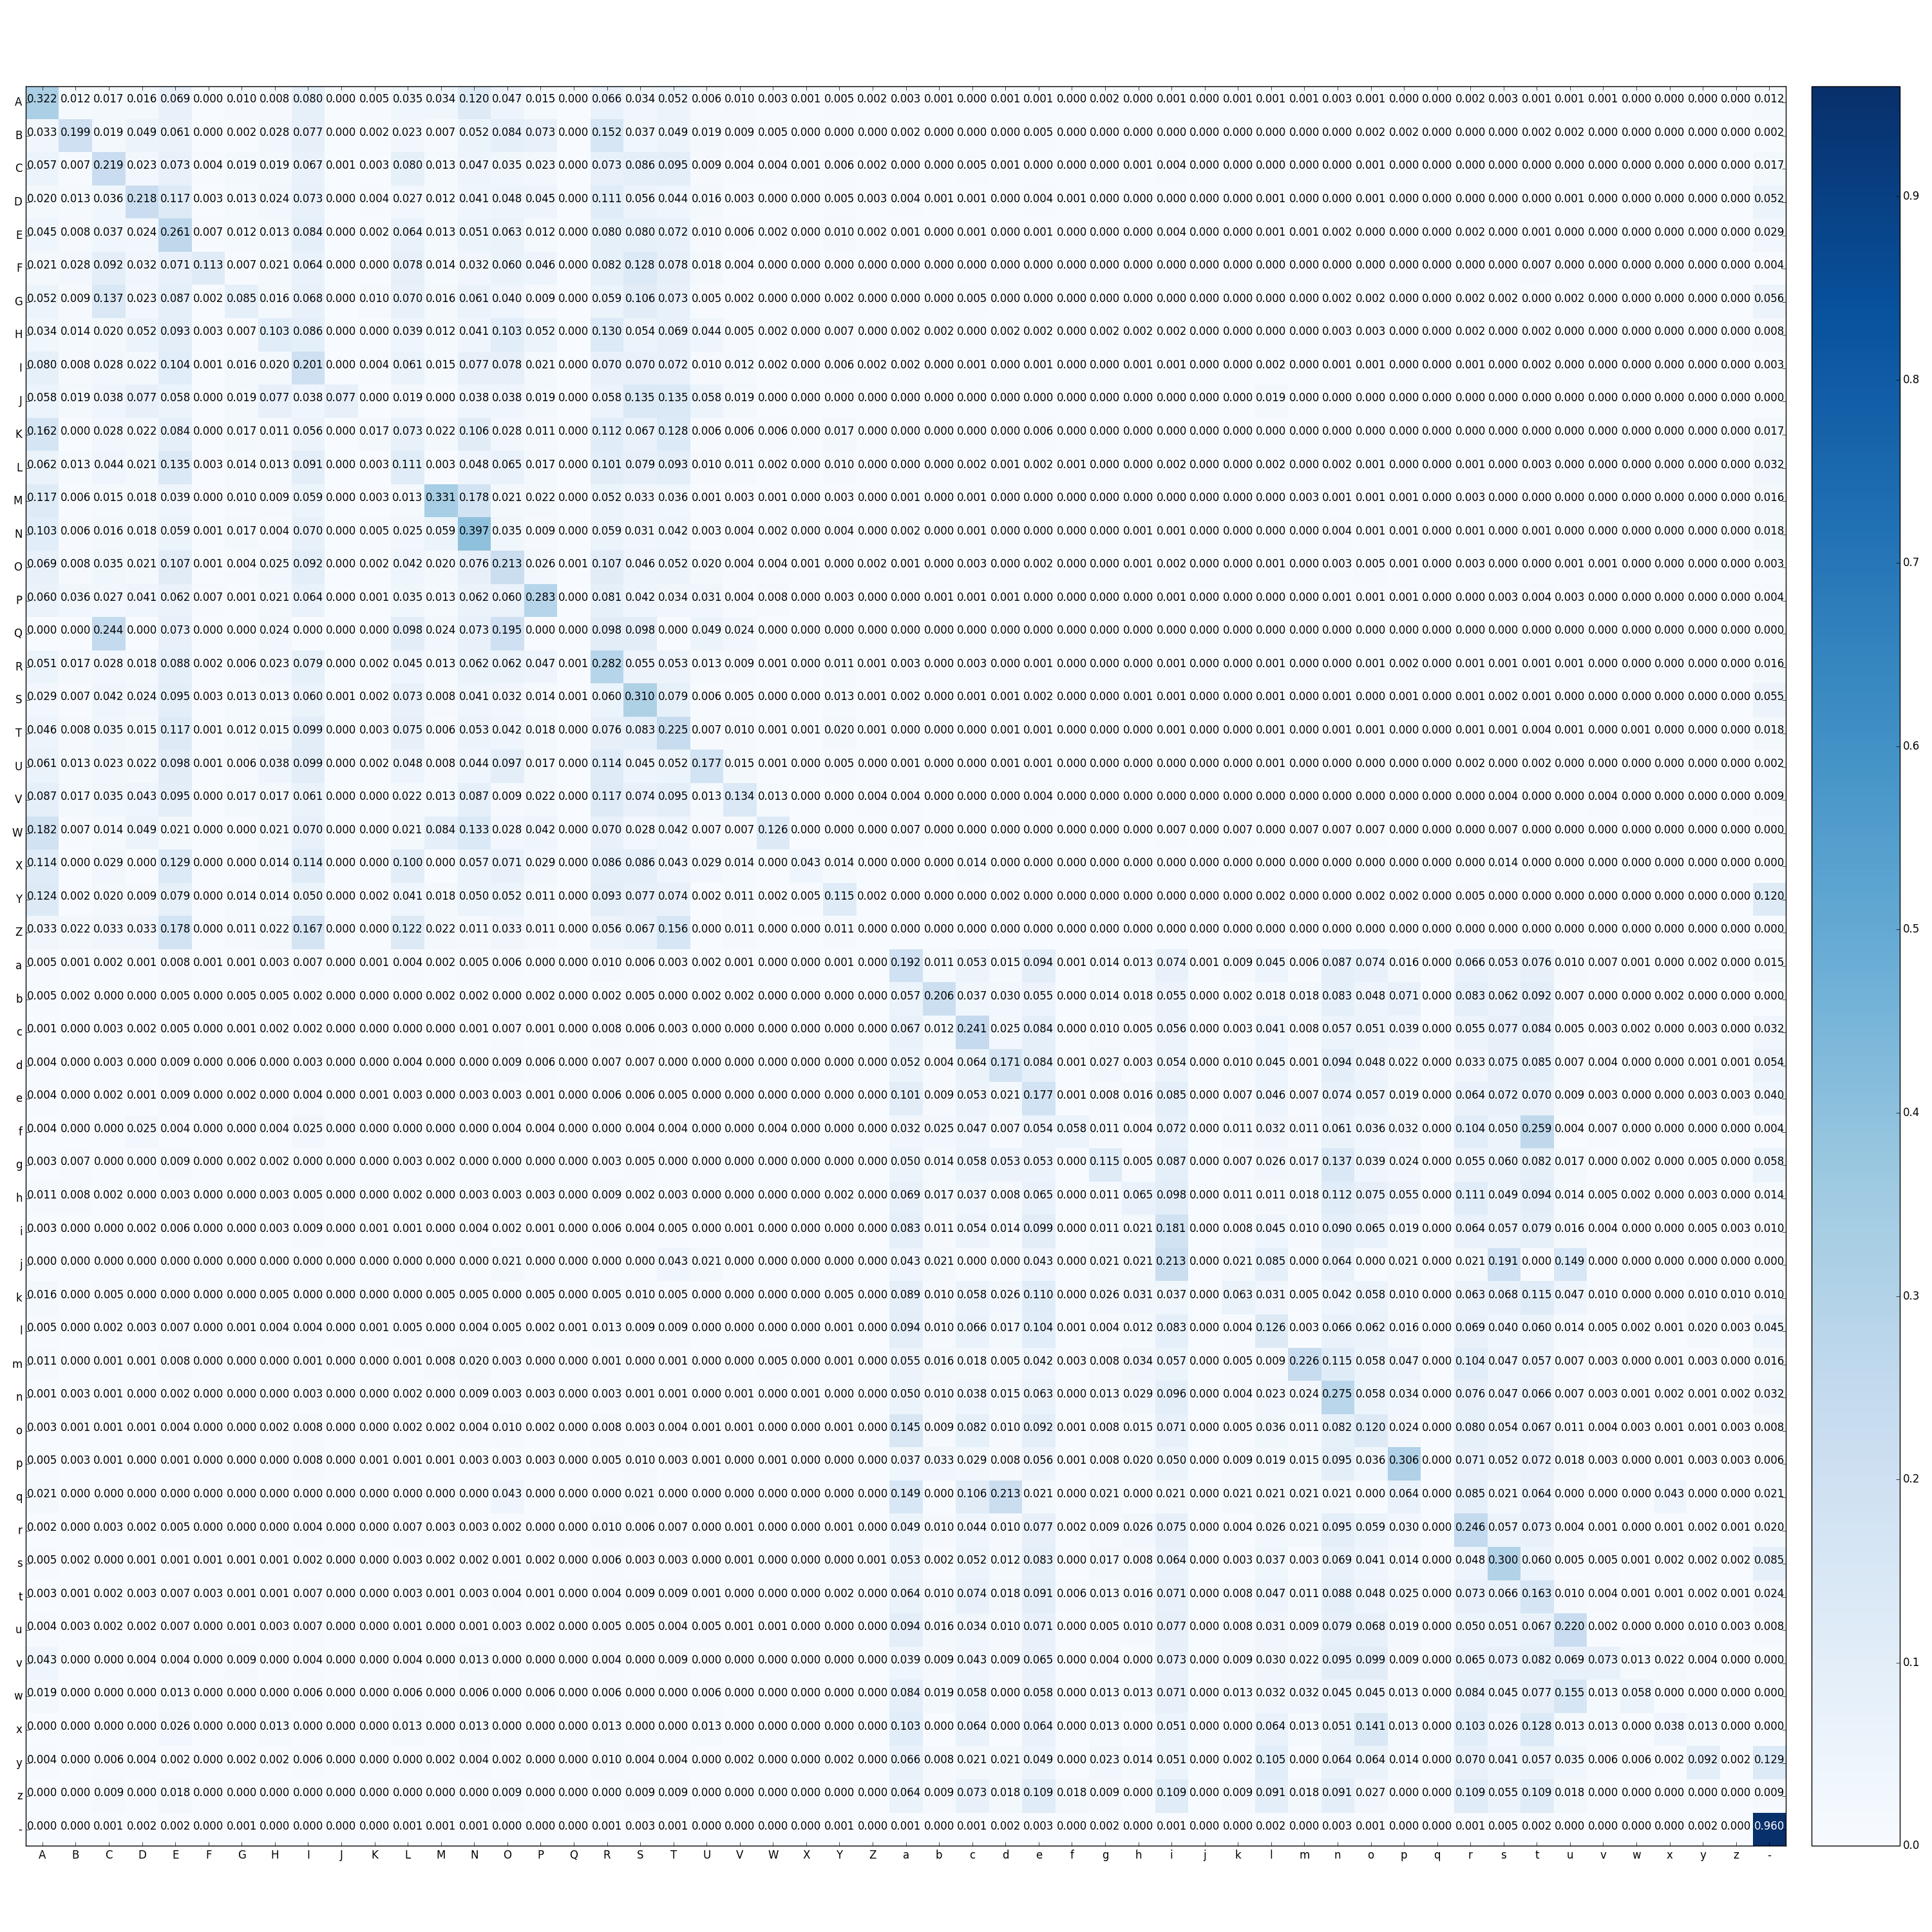
\includegraphics[width=1\textwidth]{fig/results/experiment4/encdecreg/confusion_matrix.png}
    \caption{Confusion matrix for the best {\tt EncDecReg} model on the stress test}
    \label{fig:result4_encdecreg_confusion_matrix}
\end{figure}

Shown in Figure \ref{fig:result4_encdecreg_confusion_matrix} is the confusion matrix for the best {\tt EncDecReg} model on the stress test. As depicted in this matrix, the model had a hard time classifying the labels correctly, which corresponds to its accuracy of 55\%. Despite the somewhat low accuracy, the confusion matrix shows traces of a faint diagonal line going from corner-to-corner, indicating correct classifications. In general, the model seem capable of separating the upper-cased and lower-cased letters from each other, having almost no incorrect labeling shared between the two halves of the matrix. For both groups of upper-cased and lower-cased classes, the model seem to favor a few letters in each, wrongly classifying them across a wide spectrum of other letters.

\subsection{EncDecAtt Results}
\begin{figure}[H]
    \centering
    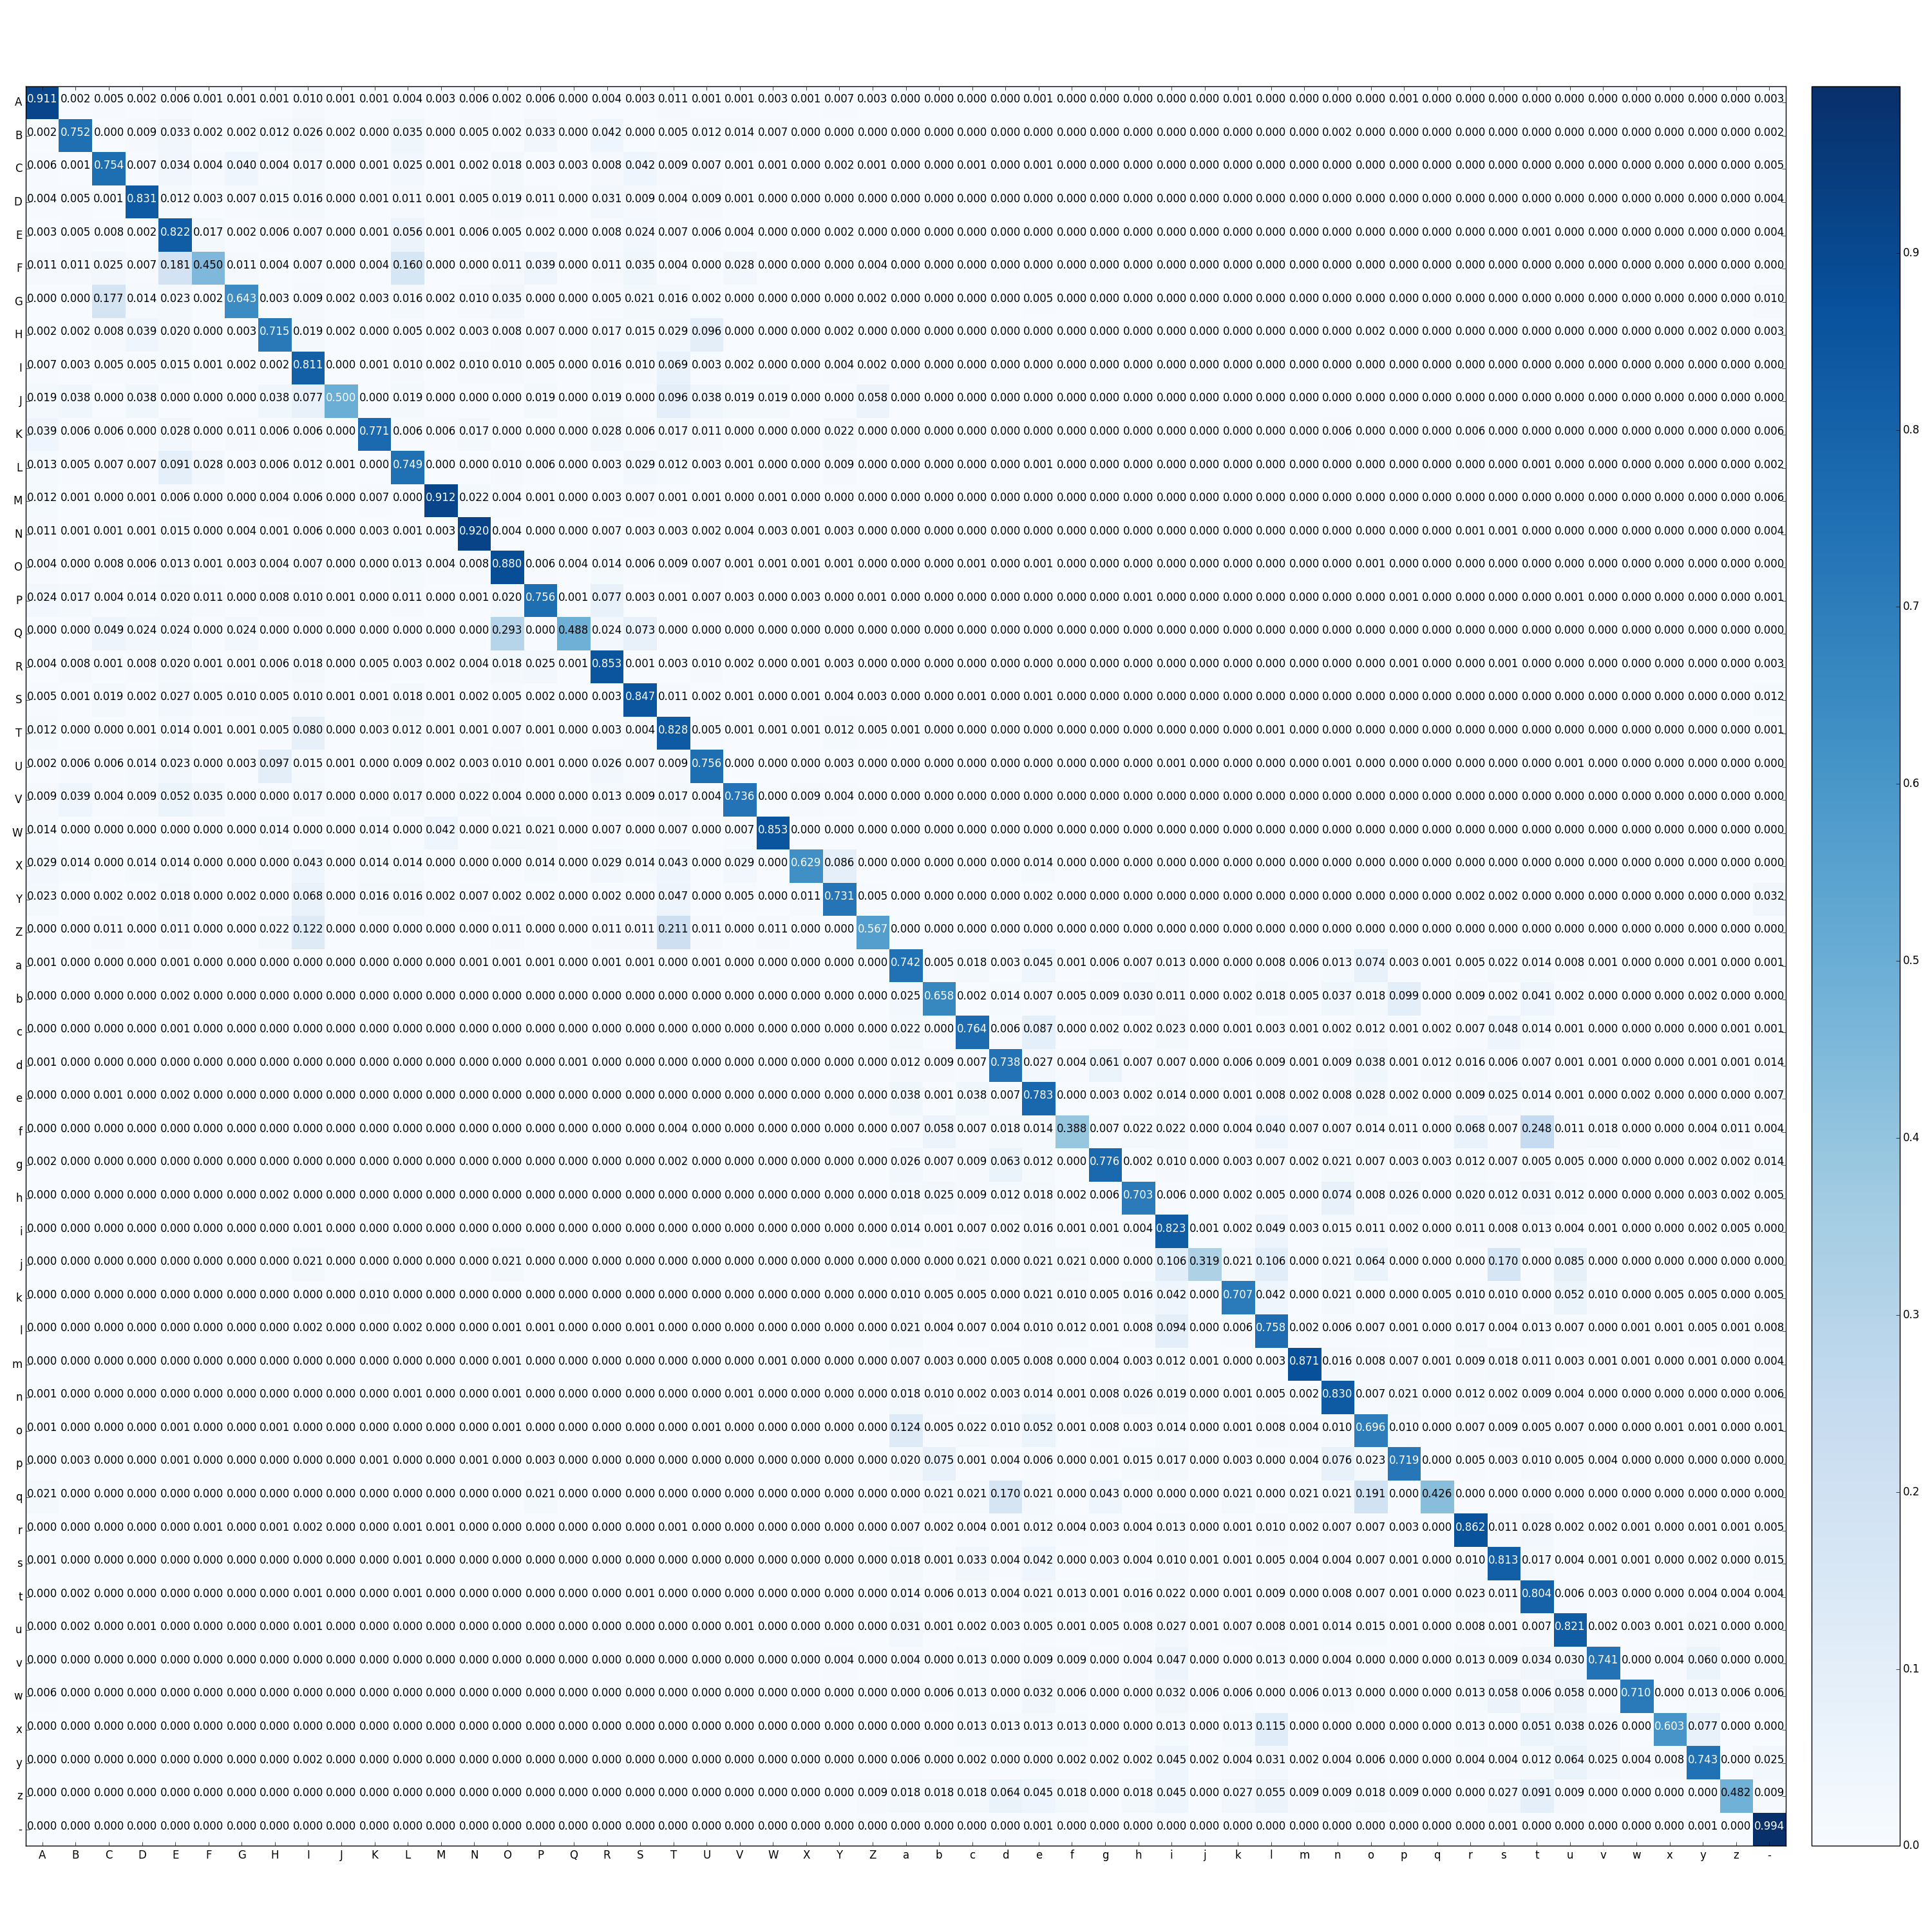
\includegraphics[width=1\textwidth]{fig/results/experiment4/encdecatt/confusion_matrix.png}
    \caption{Confusion matrix for the best {\tt EncDecAtt} model on the stress test}
    \label{fig:result4_encdecatt_confusion_matrix}
\end{figure}

Figure \ref{fig:result4_encdecatt_confusion_matrix} shows the classification matrix of the best {\tt EncDecAtt} model on the stress test. This matrix depicts a clear diagonal line from corner-to-corner, indicating that the model has been able to, for the most part, classifying labels correctly. Although there are certain labels that are mis-classified, the vart majority of labels are correctly classified, which corresponds to the accuracy of over 88\% for this model. The confusion matrix also show almost no overlap between the labels in the upper-cased and lower-cased classes, indicating that also this model was able to seperate these groups from each other. 

%%=========================================

\section{Result Discussion}
In this section, we discuss and compare the various results and models against each other. We also answer the research goals we defined earlier. The final conclusion is given in Chapter \ref{ch:conclusion}.

\subsection{General Analysis}


Results across all tests indicates several things. The {\tt VecRep} model failed to give satisfactory results, 

\subsection{Analysis In Terms of Research Questions}

\subsubsection{Ambiguity in Character Signature Sequences}
Our first research question, \textbf{RQ1}, we asked if the models were able to deal with ambiguity in the input data. In our first experiment, we used the same system configurations as shown in Table \ref{table:signature_sequence_example}, which we used to illustrate how some of the letter signatures were either identical or subsequences of another. In this table we showed that the letters C, I, J, L, T, and Y all shared the same unique signature of three black pixels. The other letters that also shared an identical signature were E and F, H and U, O and Q, and S and X. 

Comparing these sets to the confusion matrices, we can see that some of these characters were indeed those the models struggled to classify correctly. Specifically, U, I and T, F and E, as well as Q and O were problematic for both the encoder-decoder models, although their accuracy were no lower than 0.692 for the {\tt EncDegReg} model, and 0.776 for the {\tt EncDegAtt} model on any label. The most commonly wrongly classified label was an E as F, with both the models having an equal confusion of 0.18. 

These numbers indicate that there is still room for improvement, and that ambiguity may be a concern.

\subsubsection{Handling of Multiple Fonts}
Experiments have indicated that both the encoder-decoder models are able to handle more than one font, as questioned in research question \textbf{RQ2}, although the model without the attention mechanism had visible lower results than experiments carried out on datasets consisting of one font. The {\tt EncDecAtt} model was more or less unaffected by the introduction of an additional font in the first experiment. The same model also yielded good results in the stress test, where the input consisted of five different fonts. On the same test, the {\tt EncDecReg} model had much lower results, indicating that this model may be unsuitable for input with such high variety in the sequences.

\subsubsection{Handling of Noise}
Lastly, \textbf{RQ3} asked if the model(s) were able to adapt to noise and imperfect input data. Experiments have shown that the {\tt EncDecAtt} model was able to handle increasing amounts of noise, although the accuracy decreased as the noise factor increased. For a noise factor of 5\%, the accuracy decreased by a little less than 5\%, while a noise factor of 10\% decreased the accuracy by more than 28\%. This indicates that although the accuracy decay, it is really a question of how much noise is reasonable. With a noise factor of 10\%, every 10th bit may end up corrupted. If this is reasonable to expect in a real-world scenario is hard to say. We have decided to conclude this question by stating that the {\tt EncDecAtt} was able to handle noise in a satisfactory manner, although there is still a lot of room for improvements.